% !TeX root = /../Report.tex

\chapter{Introduction}\label{sec:introduction}

\section{TAVI/TAVR}\label{sec:tavi}

TAVI/TAVR stands for Transcatheter Aortic Valve Implantation/Replacement (In the following only named TAVI), which is a minimal invasive surgery meant to treat AS (Aortic Stenosis), a condition caused for the calcification of the aortic valve (Figure~\ref{img:TAVICalValve}), making it harder and thicker~\cite{tavi2013}. This condition in the valve disturbs the blood flow going into the aortic artery, making the heart work harder.\\

\begin{figure}[ht]
   \centering
   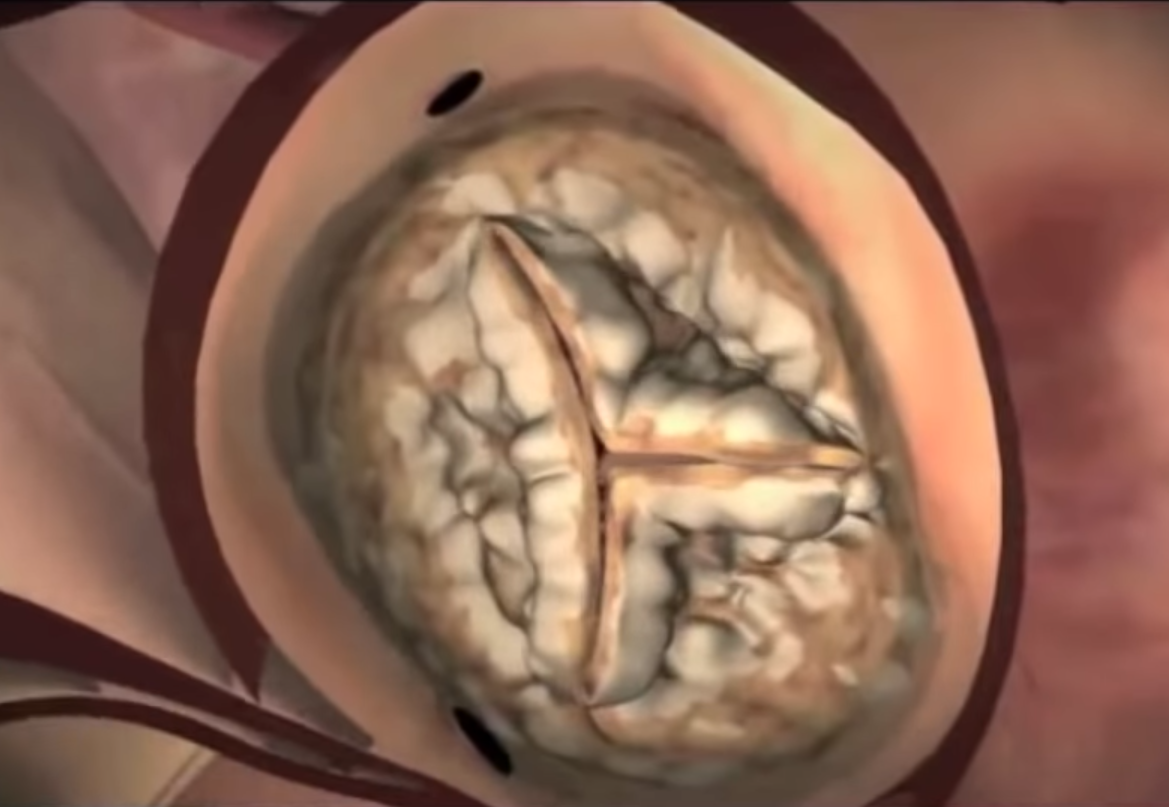
\includegraphics[width=0.6\textwidth]{img/TAVICalValve.PNG}
   \caption{Aortic valve with AS (image taken from~\protect\cite{tavivideo})}
   \label{img:TAVICalValve}
\end{figure}

TAVI surgery is performed through an incision in the groin, where a sheath is placed in order to give access to a variety of guide wires and catheters to the aortic artery. Different guide wires and catheters are used to first gain access to the aortic arch, then go through it and finally gain access to the left heart ventricle crossing the calcified aortic valve. Each one of these steps require a combination of axial and rotation movements performed by the surgeon to avoid damages in the artery and valve.\\

Once access to the left ventricle of the heart is granted, a balloon-expandable mounted on a catheter is inserted and positioned in the calcified valve. When in position, the balloon is expanded in order to retract the leaflets of the diseased valve (Figure~\ref{img:TAVIBalloon}).\\

\begin{figure}[ht]
   \centering
   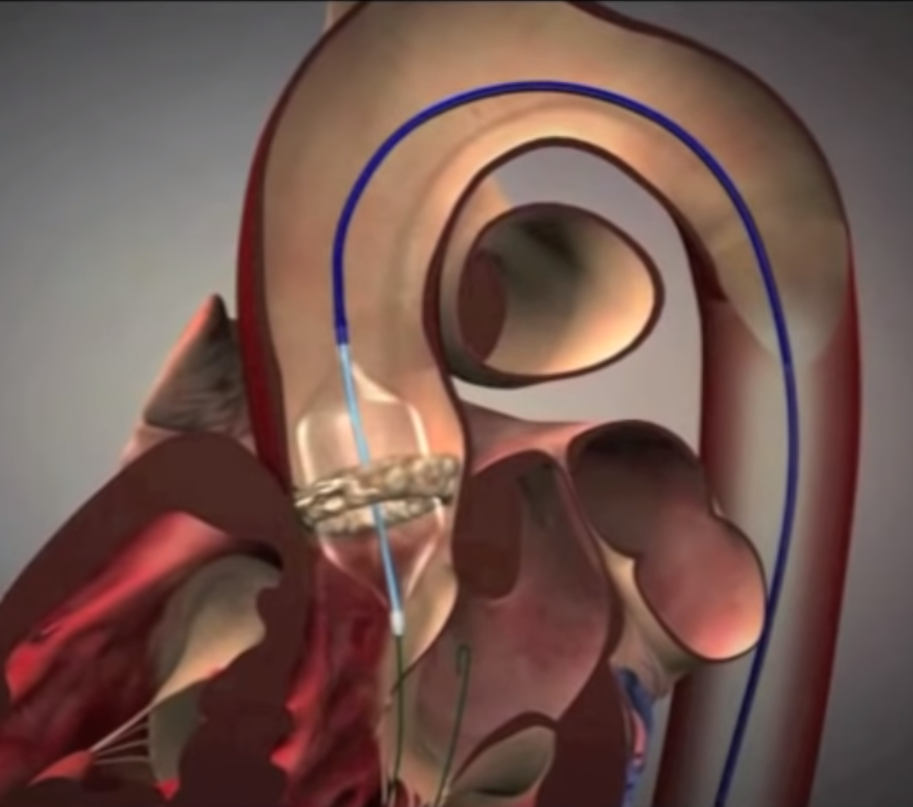
\includegraphics[width=0.5\textwidth]{img/TAVIBallon.PNG}
   \caption{Balloon catheter retracting the calcified valve (image taken from~\protect\cite{tavivideo})}
   \label{img:TAVIBalloon}
\end{figure}

Last, the new aortic valve is inserted mounted on a catheter and placed over the retracted old calcified valve. After the new valve is in position and fully expanded  (Figure~\ref{img:TAVIValve}), the leaflets start working regulating the blood flow. If the placement was successful, the catheter and guide wire are retracted and the groin incision closed.\\

\begin{figure}[ht]
   \centering
   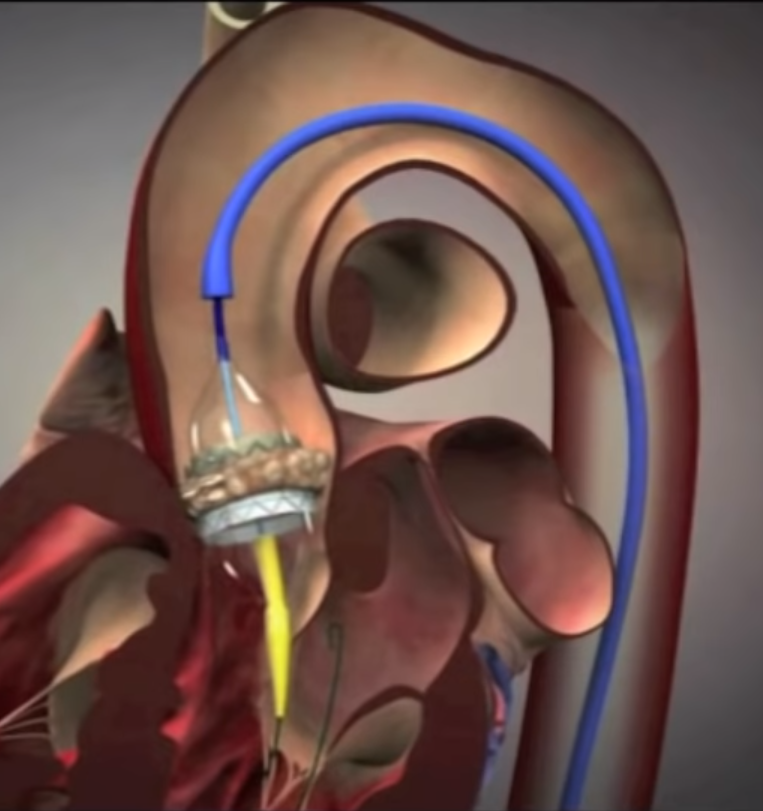
\includegraphics[width=0.5\textwidth]{img/TAVIValve.PNG}
   \caption{Artificial valve deployment (image taken from~\protect\cite{tavivideo})}
   \label{img:TAVIValve}
\end{figure}

During the whole surgery, the physicians have visual guidance help provided by fluoroscopy image (2D image), in order to track the position of the catheter and wires at any time, as well as the positioning of the balloon-expandable and the new aortic valve when being deployed.\\
\clearpage

\section{Motivation}\label{sec:motivation}

TAVI procedure has become more popular since the FDA approved, in 2016, the procedure for intermediate risk patients that present sever AS~\cite{tavi2019}, and estimates predict that numbers in North America and Europe will raise more than double (270 000 patients annually) if it is approved for low risk patients~\cite{taviprojection}.\\

Each one of these surgeries suppose a risk not only for the patients, but for every interventionalist present in the room, given that per each intervention interventionalists are exposed to a median of 5.5 mRad produced by the fluoroscopy imaging~\cite{taviradiation}, being cardiologist, the medical professionals exposed to the highest amounts of radiation~\cite{tavibrain}. Recent studies have shown that:
\begin{itemize}
 \item 	85\% of the brain tumors found in interventionalists are located on the left side of the brain, consistently with the closest side of the brain to the radiation source in the surgery room(Figure~\ref{img:operationroom})~\cite{tavibrain}.
 \item 	50\% of the interventionalists have significant posterior subcapsular lens changes, causing propensions to cataracts~\cite{tavilens}.\\
\end{itemize}

\begin{figure}[ht]
   \centering
   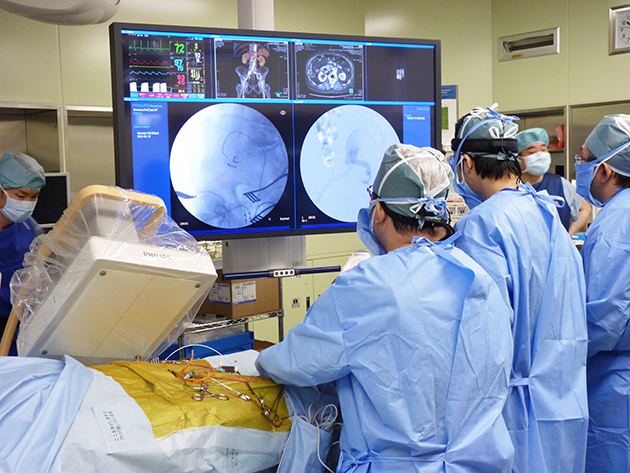
\includegraphics[width=0.7\textwidth]{img/operationroom.PNG}
   \caption{TAVI surgery room with fluroscopy on the left (image taken from~\protect\cite{taviroom})}
   \label{img:operationroom}
\end{figure}

In order to mitigate the risks inherent to radiation exposure, a common practice is wearing a leaded suit as protective equipment. These suits have to be worn at any time while the fluoroscopy imaging system is turned on. Such suits are commonly made of lead and may weight up to 7 Kgs (Figure~\ref{img:leadvest}). This additional weight may cause orthopedic issues as proven in recent studies:
\begin{itemize}
 \item  60\% have suffered spine issues after 21 years in practice ~\cite{tavihazards}.
 \item 	33\% miss work due to orthopedic issues~\cite{tavimissed}.\\
\end{itemize}

\begin{figure}[ht]
   \centering
   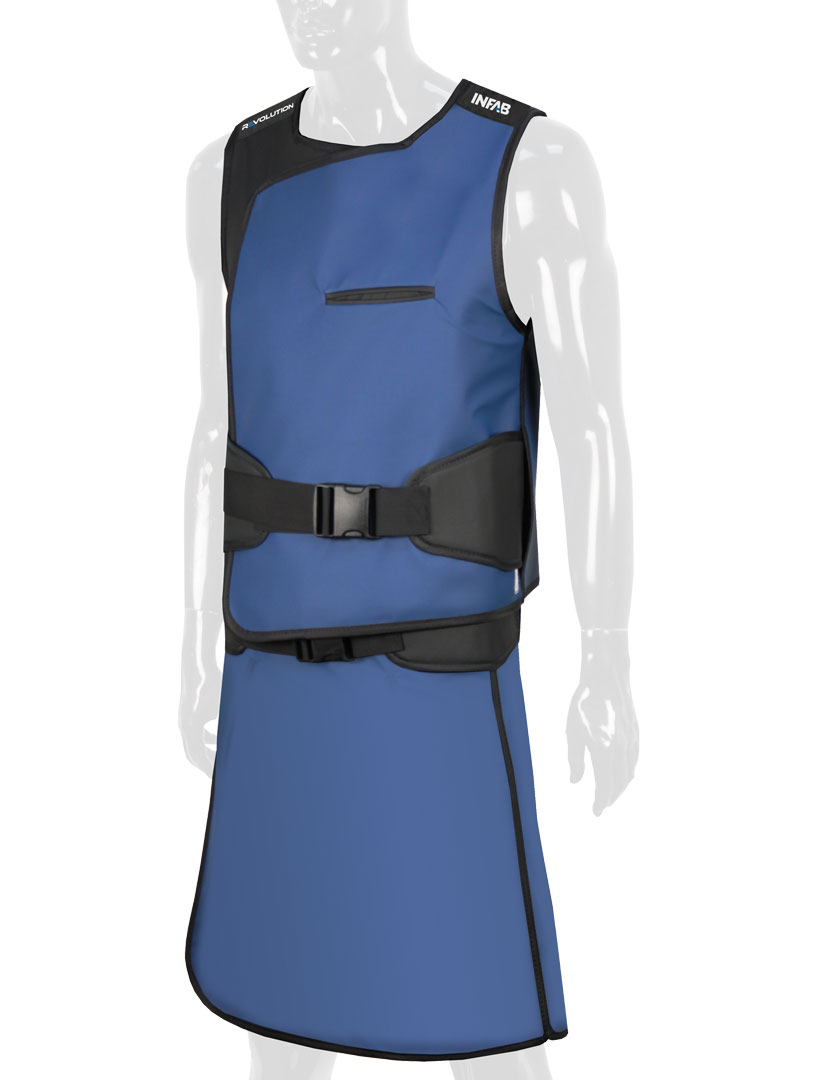
\includegraphics[width=0.4\textwidth]{img/leadvest.PNG}
   \caption{Lead suit commonly used for TAVI procedure (image taken from~\protect\cite{tavivest})}
   \label{img:leadvest}
\end{figure}

This is why we believe TAVI procedures should be performed assisted by a teleoperated robot, allowing this way to set the interventionalists away from the radiation source. Although many teleoperated robots already exist in the market for surgeries involving the use of catheters, none has been developed specifically for TAVI and its specific needs.\\
\clearpage

\section{Teleoperation}\label{sec:teleoperation}

A teleoperated surgical robot allows the surgeon to be located away from the operation table, and thus, for TAVI procedure, away from the radiation source. Teleoperation has proven in similar surgeries to reduce the radiation in patients on 17\%~\cite{pci} and to reduce as well the exposure to the primary surgeon in 95\%~\cite{pcisafety}, beside the orthopedic benefits implied by not wearing the lead suits at all times during the surgery.\\

As depicted in Figure~\ref{img:teleoperation} the working station for the surgeon can be located away from the operation table, together with the fluoroscopy imaging screen and the master device, which may be actuated for haptic feedback, giving the surgeon another dimension given that the visual cues are poorly displayed in a black and white 2D image.\\

\begin{figure}[ht]
   \centering
   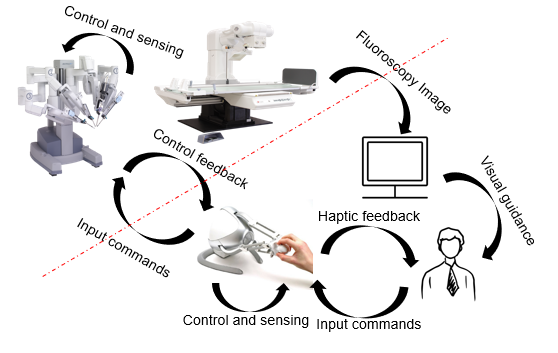
\includegraphics[width=0.8\textwidth]{img/teleoperation.PNG}
   \caption{Teleoperation diagram}
   \label{img:teleoperation}
\end{figure}

\section{Objective}\label{sec:objective}

This thesis work intends to find the most suitable master device type for a TAVI/TAVR teleoperated robot, capable not only of controlling the 2 DOF (translation and rotation) of the different catheters and guide wires used during the intervention, but also capable to allow the surgeons to succeed in the most complex maneuvers involving both DOF movements at the same time when crossing the aortic valve (Long maneuver times at this state increases the risk of cerebral embolism)~\cite{raptech}~\cite{anatomic} and to perform accurate movements to position the artificial valve before deployment, mitigating this way paravalvular leak complications present in 8\% of the TAVI procedures~\cite{pvl}~\cite{pvl2}.\\

